\documentclass[10pt,a4paper]{article}
\usepackage[utf8]{inputenc}
\usepackage[russian]{babel}
\usepackage[OT1]{fontenc}
\usepackage{amsmath}
\usepackage{amsfonts}
\usepackage{amssymb}
\usepackage{makeidx}
\usepackage{graphicx}
\usepackage{tikz}

\usepackage{graphicx}
\usepackage{caption}


\usepackage{float}
\floatstyle{boxed}
\restylefloat{figure}

\author{Максим Борисяк}
\title{Дипломная работа}
\makeindex

\newtheorem{defen}{Определение}

\newcommand{\stock}{\text{STOCK}}
\newcommand{\source}{\text{SOURCE}}
\newcommand{\initial}{\text{INITIAL}}

\newcommand{\FA}{F\!A}

%\textheight = 720pt
%\textwidth = 500pt

%\hoffset = -25mm
%\voffset = -30mm

\begin{document}

\maketitle

\section{Введение}

Введение.

\subsection{Мотивация}
Мотивация

\subsection{Базовые понятия и определения}
В данном разделе будут введены базовые понятия, используемые в данной работе, в том числе,
понятия атомарного блока, составного блока, потока данных, автомата Мили соответствующего блоку и так далее.

Основной единицей потока данных является атомарный блок.
\begin{defen}
  \textbf{Шаблоном атомарного блока} $s$ (сокращенное от англ. \textit{scheme} --- схема) назовем кортеж имеющий два не пересекающихся набора портов: \textit{входной} и \textit{выходной}.
  $s = (\FA, I, O)$, где:
  \begin{itemize}
    \item $I = \{b^I_i \vert i = \overline{1, N_I}, N_I \in \mathbb{N}\}$ --- конечное множество уникальных входных портов;
    \item $O = \{b^O_i \vert i = \overline{1, N_O}, N_O \in \mathbb{N}\}$ --- конечное множество уникальных выходных портов;
    \item $\FA$ --- конечный автомат Мили, смысл и структура которого будет обсуждаться в дальнейшем.
  \end{itemize}
\end{defen}
Сразу заметим, что не любая тройка $(\FA, I, O)$ является шаблоном атомарного блока, так как $\FA$ должен
соответствовать множествам $I$ и $O$.

Стоит отметить, что природа множеств $O$ и $I$ совершенно не важна, например, они могут быть просто множеством чисел: $I, O = \{i \in \overline{1, \dots, N_{I, O}}\}$,
на практике часто используют строки для именования портов, так как порты могут существенно различаться по смыслу, а их именование помогает избежать путаницы.
Последний подход используется в рисунках.

\begin{defen}
  \textbf{Атомарным блоком} $b = (id, s, state)$, где:
  \begin{itemize}
    \item $id$ --- уникальный для всех блоков идентификатор;
    \item $s$ --- шаблон атомарного блока;
    \item $state \in S$, где $S$ множество состояний $\FA_s$ --- текущее состояние атомарного блока.
  \end{itemize}
\end{defen}

Идентификатор $id$ введен из-за следующих соображений: в потоке данных некие блоки могут описываться одним и тем же шаблоном, находиться в одном и том же состоянии,
но все равно будут являться различными блоками, в частности, могут перейти в различные состояния в следующие моменты времени либо могут иметь в потоке данных разный смысл и,
соответственно, иметь различные соединения с другими блоками.

В реальных системах для построения и запуска потока данных шаблон атомарного блока представляется в виде подпрограммы или модуля
(функции, класса некого объектно-ориентированного языка программирования, динамической библиотеки), который используя данные некого набора своих входных портов,
вычисляет и записывает данные в свои выходные порты. В таком случае, атомарный блок представляется в виде набора внутренних переменных,
либо (что тоже самое) в виде экземпляра класса объектно-ориентированного языка программирования соответствующего шаблону.
В такой интерпретации некую вычислимую функцию $f(x_1, x_2, \dots, x_n)$ можно представить в виде шаблона блока $b_f$
с входными портами $x_1, x_2, \dots, x_n$ и одним выходным портом $F$, который при получении данных со всех входных портов
выписывает значения функции $f(x_1, x_2, \dots, x_n)$ в порт $F$.

На рисунке \ref{map} схематично изображен шаблон блока \textit{Loop}, для которого $inputs(Loop) = \{xs, f\}$, $outputs(Loop) = \{fs, x\}$.

\begin{figure}[H]
  \centering

  \begin{subfigure}[b]{0.2\textwidth}
	
  \end{subfigure}
  ~
  \begin{subfigure}[b]{0.7\textwidth}
    \centering
    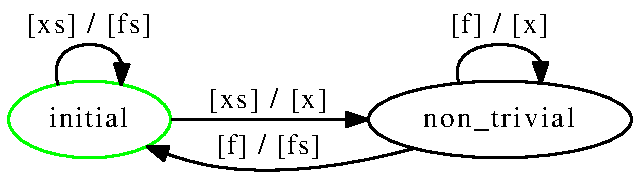
\includegraphics[width=\textwidth]{map_fa.pdf}
    \caption{Автомат Мили шаблона \textit{Loop}}
    \label{map:fa}
  \end{subfigure}
  
  \caption{Схематичное изображение шаблона блока \textit{Loop} (a) и соответствующего ему конечного автомата Мили (b).}
  \label{map}
\end{figure}

Основной структурой для построения схемы потока данных является составной блок.

\begin{defen}
 \textbf{Шаблоном составного блока} будем называть кортеж $c = (B, E, I, O)$, где:
 \begin{itemize}
    \item $B$ - конечное множество блоков (сразу заметим, что блоком может являться и составной блок, определенный ниже).
    \item $E$ - множество ребер вида $e_b = (b_1, b^O_{1}, b_2, b^I_{2})$, $b_1, b_2 \in B$, $b^O_{1} \in outputs(b_1), b^I_{2} \in inputs(b)$,
                либо вида $e_I = (c^I, b, b^I)$, $e_O = (b, b^O, c^O)$, где $b \in B$, $b^I \in inputs(b)$, $b^O \in outputs(b)$, $c^O \in O$, $c^I \in I$.
                Множества ребер $e_b$ будем обозначать как $E^B$, $e_I$ и $e_O$ как $E^I$ и $E^O$ соответственно.
    \item $I$, $O$ - наборы входных и выходных портов (по аналогии с атомарным блоком).
  \end{itemize}
\end{defen}

В дальнейшем в выражениях вида $I_c$ или $O_c$ нижний индекс будет указывать на схему блока, которому принажлежат эти множества.

Для анализа внутренней структуры удобно рассматривать иное представление шаблона составного блока $c$, добавляя фиктивные блоки $\stock$, $I_{\stock} = O_{\stock} = O_c$,
  и $\source$, $I_{\source} = O_{\source} = I_c$:
$$\hat{E}^I = \{(\source, \source^O, b, b^I) \vert (\source^O, b, b^I) \in E^I\}$$
$$\hat{E}^O = \{ (b, b^O, \stock, \stock^I) \vert (b, b^O, \stock) \in E^O \}$$
$$\hat{c} = (B \cup \{\stock, \source\}, E^B \cup \hat{E}^I \cup \hat{E}^O)$$
В этом случае шаблон составного блока $\hat{c}$ описывается графом с ребрами вида $(u, u^O, v, v^I)$,
а входными и выходными портами всего шаблона считаются входные и выходные порты блоков $\source$ и $\stock$.
На рисунке \ref{example} изображен примеры шаблонов составных блоков во втрой интерпретации.

\begin{defen}
  \textbf{Составным блоком} будем называть $b = (id, c = (B, E, I, O), state)$, где
  \begin{itemize}
    \item $id$ --- уникальный идентификатор;
    \item $c$ --- шаблон составного блока;
    \item $state \in \Sigma \times 2^E = \prod S(B) \times 2^E \times 2^B$ - текущие состояние составного блока, включающее
          состояние каждого блока (подпространство $\Sigma = \prod S(B)$), активную волну ($\omega \in \Omega = 2^E$) и
          множество активных блоков ($\vartheta \in \Theta = 2^B$), смысл которых будет пояснен позже.
  \end{itemize}
\end{defen}

\begin{figure}[H]
  \centering
  \begin{subfigure}[b]{0.3\textwidth}
    \centering
    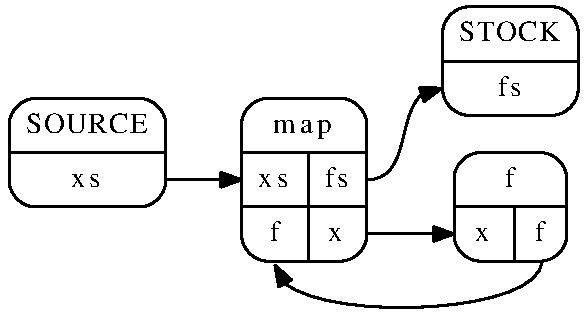
\includegraphics[width=\textwidth]{example_cg.pdf}
    \caption{Шаблон составного блока}
    \label{example:composite}
  \end{subfigure}
  ~
  \begin{subfigure}[b]{1.0\textwidth}
    \centering
    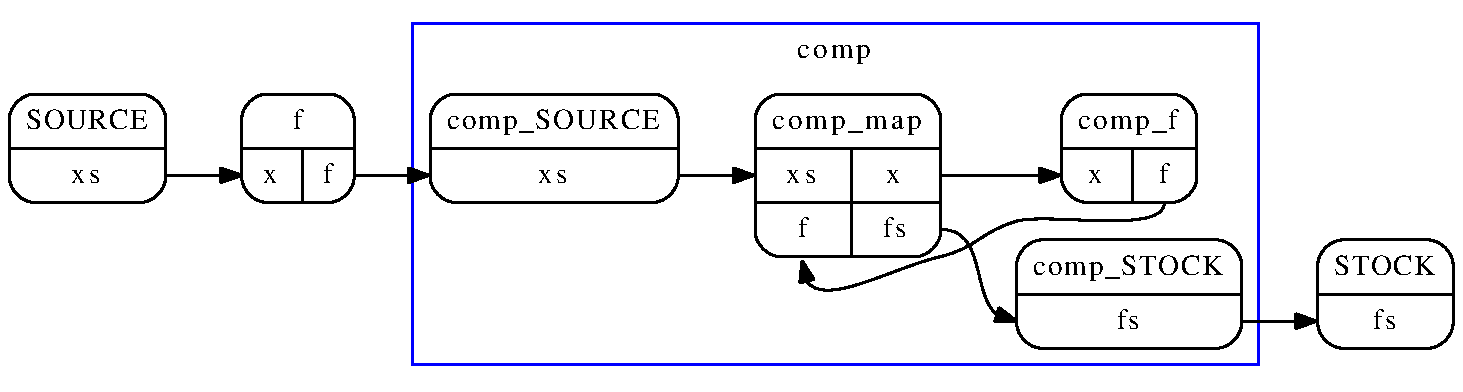
\includegraphics[width=\textwidth]{cc_cg.pdf}
    \caption{Шаблон супер-составного блока. Внутри рамки показана структура шаблона внутреннего блока.}
    \label{example:supercomposite}
  \end{subfigure}
  
  \caption{ Примеры графов составного и супер-составного блока.}
  \label{example}
\end{figure}

Заметим, что составной блок (в исходной интерпретации) внешне не отличим от атомарного блока.
Поэтому под понятием блока мы будем подразумевать либо атомарный блок, либо составной блок,
различая их только в том случае, когда речь заходит о их внутреннем строении. Составной блок может включать в себя другие составные блоки.
На рисунке \ref{example:supercomposite} показан пример составного блока, включающего другой составной блок, иными словами супер-составного блока.
На практике свойство вложенности реализует принцип модульности программ --- модулем в нашем случае будет шаблон составного блока.
Бессмысленно рассматривать случаи, в которых структура составного блока бесконечна в глубину, например,
в случае когда шаблон составного блок содержит содержит блок того же шаблона. Поэтому в дальнейшем, мы будем рассматривать только составные блоки конечной глубины.

Заметим, что составным блоком можно описать любую программу, имея в распоряжении необходимые примитивы --- шаблоны атомарных блоков,
реализующие Тьюринг-полную систему операций. Доказательства этого факта выходит за задачи данной работы и может быть найдено, например, в работе \textbf{[???]}.
Из-за достаточной выразительности составного блока, схему потока данных мы определим просто как схему некого составного блока.

Теперь неформально поясним схему работы составного блока и смысл его структуры.
В общепринятых определениях потока данных ребра графа шаблона составного блока обозначают зависимость по данным, то есть ребро $e = (u, u^O, v, v^I)$ представляет собой
\textit{FIFO}-канал соединения между портами блоков и
можно словесно интерпретировать следующим образом: блок $v$ в качестве данных из входного порта $v^I$ должен использовать данные выходного порта $u^O$ блока $u$ при их наличии.
Блок $u$ после завершения своей работы может "испустить данные по порту $u^O$", которые мгновенно "переносятся" на все ребра из $u^O$ блока $u$,
если эти ребра свободны.
Когда блоку $v$ требуются данные из порта $v^I$, данные с ребра $e$ мгновенно "переносятся" в соответствующий порт блока. В этом и есть смысле подпространства $\Omega = 2^E$
в определении состояния составного блока --- \textit{активной волной} $\omega$ мы назовем множество ребер, которые содержат на данный момент данные.

Однако такая схема работы составного блока порождает множество неопределенностей в работе некоторых составных блоков, например, неопределенность выбора ребра для "поглощения" данных из определенного порта (состояние гонки).
Неопределенности подобного рода мы будем рассматривать как ошибки, обнаружению которых посвящена часть данной работы. Такого рода неодназначности, особенно в реальных системах,
то есть в условиях неопределенного времени вычислений блоков и их параллельного выполнения, может привести к совершенно иному ходу потока данных, нежели было задумано автором потока данных.
Поэтому наличие подобного рода неопределенностей (состояний гонки) говорит скорее о неправильном построении схемы потока данных, чем о некой задумке автора потока данных.
Более подробно и строго об неоднозначностях в поведении потока данных будет идти речь ниже.
Стоит заметить, что подобного рода неоднозначности возникают и в процессе определения сетей процессов Кана,
которые решаются наложением условий на правила поглощения и испускания, а также на класс функции процесса.
Мы же пойдем другим путем, накладывая ограничения лишь на граф шаблона потока данных, оставляя подпрограммы и правила поглощения каждого шаблона блока без ограничений.
В нашем случае правила поглощения состоят в том, что формально блок может поглотить любые доступные данные из любых портов по любым ребрам,
но будем расценивать любые возможные неоднозначности как ошибку построения потока данных.

Выше были рассмотрены определения и термины, которые с той или иной точностью присутствуют практически во всех моделях потока данных.
В данной работе мы абстрагируемся от данных, а значит нас интересуют только возможные зависимости наборов входных портов от набора выходных портов,
иными словами только качественное поведение блоков. Оказывается, конечный автомат Мили хорошо подходит для описания качественного поведения блоков.
Заметим, что в данной работе используется не стандартное определение автомата Мили, а его недетерминированные аналог.
Дадим теперь строгое определение конечного автомата Мили.

\begin{defen}
  \textbf{Конечный автомат Мили} --- кортеж $\FA = (S, s_0, \Sigma, \Lambda, E)$, где:
  \begin{itemize}
    \item $S$ --- конечное множество состояний;
    \item $s_0 \in S$ --- начальное состояние;
    \item $\Sigma$ --- входной алфавит;
    \item $\Lambda$ -- выходной алфавит;
    \item $E \subseteq S \times \Sigma \times \Lambda \times S$ --- отношение возможных переходов.
  \end{itemize}
\end{defen}

Для удобства будем рассматривать функцию конечного автомата Мили $\FA = (S, \cdot, \Sigma, \Lambda, E)$:
$\FA(p, \sigma) = \{(\lambda, q, \sigma') \vert (p, \sigma', \lambda, q) \in E, \sigma' \subseteq \sigma\}$.
Стоит обратить внимание на нестандартную форму данной функции. Далее символами в алфавитах $\Sigma$ и $\Lambda$ будут множества, поэтому функция по текущему состоянию и входному множеству возвращает множество троек вида:
выходной символ-множество, новое состояние и поглощенное множество.

Конечный автомат Мили выполняет преобразование последовательности входных символов из алфавита $\Sigma$ в последовательность символов в алфавите $\Lambda$.
Вернемся теперь к определению шаблона атомарного блока. В данной работе мы абстрагируемся от конкретного алгоритма преобразования входных данных в выходные
и преобразования внутреннего состояния блока. Вместо этого мы будем описывать лишь качественное поведение алгоритма автоматом Мили $\FA$, в котором входной алфавит
$\Sigma = 2^I \setminus \varnothing$ (запрещается запуск по пустому набору входных портов),
а выходной алфавит $\Lambda = 2^O$, иными словами ребро $e = (u, is, os, v)$ автомата $\FA$ описывает возможный переход из состояния $u$ в состояние $v$,
при считывании данных из портов $is$ и выписывании данных в порты $os$ (именно поэтому функция $\FA$ имеет странный на первый взгляд вид).
На практике подпрограмма реализующая логику атомарного блока может иметь значительное количество внутренних состояний,
однако, для наших целей важны лишь группы таких внутренних состояний, которые описывают возможное поведение на определенном наборе данных из входных портов.
Более того практически во всех системах построения и запуска потока данных подпрограмма описывающая блок имеет детерминированное поведение.
Неизбежный недетерминизм в автомате Мили, описывающий блок, возникает из-за исключения из рассмотрения самих данных,
так как при разных значениях на одном и том же наборе портов из одного состояния, блок может перейти в различные конечные состояние,
даже выписав при этом данные в один и тот же набор портов.

На рисунке \ref{map:fa} изображен автомат Мили для шаблона атомарного блока $Loop$, описывающего цикл. Поясним эту схему.
Изначально блок с шаблоном $Loop$ находиться в состоянии \textit{initial}.
Далее он может считать из порта \textit{xs} начальные параметры цикла (например, некую коллекцию данных).
Если условие выхода из цикла изначально выполнено (например, пустая коллекция), то блок переходит в прежнее состояние выписав в порт \textit{fs}.
Иначе, блок отправляет данные по порту \textit{x} переходя в состояние \textit{non\_trivial}. В состоянии \textit{non\_trivial} блок имеет не тривиальное внутреннее состояние,
например, остаток коллекции. В этот состоянии блок ожидает поступление преобразованных некой внешней функцией данных на порт \textit{f}.
И в этом случае существует два варианта перехода, в зависимости от выполнения условия выхода из цикла:
$(non\_trivial, \{f\}, \{x\}, non\_trivial)$ и $(non\_trivial, \{f\}, \{fs\}, trivial)$ для случаев продолжения цикла и выхода из него соответственно.

Конечный автомат Мили может быть также определен для составного блока. Единственное отличие от автомата Мили для атомарного блока состоит в том, что
зная все автоматы внутренних блоков, можно вычислить автомат составного блока как будет показано ниже.

\subsubsection{Алгоритм работы потока данных}
Теперь опишем алгоритм вычисления потока данных, представленного в виде составного блока $c$ со схемой
$C = (\hat{B}_c = B_c \cup \{\source, \stock\}, \hat{E}_c= E_c \cup E^I_c \cup E^O_c)$ в представлении графа.
Мы будем рассматривать вычисление потока данных в предположении,
что время работы блока может быть абсолютно любым (но конечным) при любых условиях, что полностью соответствует реальным потокам данных.
В таком случае нас прежде всего будет интересовать всевозможные поведения потока данных с точки зрения относительных расположений времен запуска и завершения любого блока.
Введем модельное время $t \in \mathbb{Z}_+$.
Каждое множество, связанное с состоянием системы в момент времени $t$, снабдим верхним индексом, например, $\omega^t \in \Omega_c$.

\begin{defen}
  Определим некоторые вспомогательные функции.
  \begin{eqnarray*}
    O_v(\omega) & = & \{v^O \vert (v, v^O, \cdot, \cdot) \in \omega\}, \\
    I_v(\omega) & = & \{v^I \vert (\cdot, \cdot, v, v^I) \in \omega\}, \\
    \Delta_{O, v} & = & \{(v, v^O, \cdot, \cdot) \in E_c \vert v^O \in O\}, \\
    \Delta_{I, v} (\omega) & = & \{\tilde \omega_{I, v} \subseteq \omega \}, \; \forall \tilde \omega_I \forall v^I \in I \exists ! e \in \omega_I: e = (\cdot, \cdot, v, v^I)
  \end{eqnarray*}
\end{defen}
Последняя функция возвращает множество вариантов поглощения по набору входных портов $I$ блока $v$.

\begin{defen}
  Фронтом $\Psi_c (\omega, s)$ активной волны $\omega = \{(u, u^O, v, v^I)\} \in \Omega_c$ в состоянии $(s = (s_{u_1}, s_{u_2}, \dots, s_{u_m}), \omega, \cdot)$
  назовем подмножество блоков $\Psi_c (\omega, s) \subseteq B_c$, такое что:
  $$\Psi_c (\omega, s) = \{ v \in B \vert \FA_v(s_v, I_v(\omega)) \neq \varnothing\}$$
\end{defen}
Иными словами, фронт активной волны в заданном состоянии --- множество блоков, которые могут быть запущенны на следующем шаге.

\begin{defen}
  Семейство $\pi^t_v \in E_v, \; \FA_v = (\cdot, \cdot, E_v, \cdot)$ показывает текущий переход, который совершает блок $v$ в момент времени $t$.
\end{defen}
Заметим, что значение $\pi^t_v$ имеет смысл только для работающих на шаге $t$ блоков.

\begin{defen}
  Условием излучения назовем $\zeta(\omega^t, \omega^O) \Leftrightarrow (\omega^O \cap \omega^t = \varnothing)$.
  Также определим семейства $\zeta^t_v$:
  $$\zeta^t = \{ v \in B_c \vert zeta(\omega^t, \omega^O_v) \}$$
  $$\omega^O_v = \{ e \in E_c \vert e = (v, v^O, \cdot, \cdot), v^O \in O^t_v \}, \; (\cdot, O^t_v, \cdot, \cdot) \in \pi^t_v$$
\end{defen}
Условие излучение звучит довольно просто: блок может излучить, если все ребра соединенные с выходным набором портов свободны.

Пусть $\phi^t \subseteq \vartheta^t$ --- множество блоков, которые закончат работу после шага $t$. Для любого времени это множество может быть произвольным подмножеством $\vartheta^t$.
Однако для любого семейства этих множеств должно выполняться условие конечной работы блока: $\forall t \forall b \in \theta^t \exists \tau > t: b \in \phi^{\tau}$.

Так же для удобства введем обозначение для любого множества $A_c$ блоков из $B_c$ --- $A_c(v) \Leftrightarrow v \in A_c, v \in B_c$.

Теперь выпишем алгоритм преобразования потока данных в виде условий на переходы каждого блока из одного множества в другое.
В каждый момент времени блок $v$ может находиться в одном из трех состояний (множеств): свободен ($v \in \xi^t$), работает($v \in \theta^t$), заблокирован($v \in \chi^t$).
Время работы блоков задается $\phi^t \subseteq \vartheta^t$ --- множеством блоков, которые закончат работу после шага $t$. Для любого времени это множество может быть произвольным подмножеством $\vartheta^t$. Однако для любого семейства этих множеств должно выполняться условие конечной работы блока: $\forall t \forall b \in \theta^t \exists \tau > t: b \in \phi^{\tau}$.
Эти состояние взяты из реальных систем запуска потоков данных и служат для интуитивного понимания модели. В дальнейшем, однако, мы избавимся от этих состояний.
Также введем семейства  --- переход автомата Мили блока, который совершает блок в текущий момент.

\begin{eqnarray}
  % Free and can not be launched => Free
  \xi^t(v) \wedge \neg \Psi_c(\omega^t, s^t)(v) & \Rightarrow &
    \begin{cases}
      \xi^{t + 1}(v), \\
      s^{t + 1}_v = s^t_v, \\
      \omega^t_{I, v} = \omega^t_{O, v} = \varnothing
    \end{cases} \label{freetofree} \\
    % Free and can be launched => Work
  \xi^t(v) \wedge \Psi_c(\omega^t, s^t)(v) & \Rightarrow &
    \begin{cases}
      \theta^{t + 1}(v), \\
      s^{t + 1}_v = s^t_v, \\
      (\cdot, \cdot, I^t_v) \in \FA_v(s^{t}_v, I_v(\omega^t)), \\
      \pi^{t + 1}_v \in \{ (s^t_v, I^t_v, \cdot, s^{t + 1}_v) \in E_v\}, \\
      \omega^t_{I, v} \in \Delta_{I^t_v, v}(\omega^t), \\
      \omega^t_{O, v} = \varnothing
    \end{cases} \label{freetostart}
\end{eqnarray}

\begin{eqnarray}
  % Work and will not finish => Work
  \theta^t(v) \wedge \neg \phi^t(v) & \Rightarrow &
   \begin{cases}
     \theta^{t + 1}(v), \\
     s^{t + 1}_v = s^t_v, \\
     \pi^{t + 1}_v = \pi^t_v, \\
     \omega^t_{I, v} = \omega^t_{O, v} = \varnothing
   \end{cases} \label{worktowork} \\
   % Work, will finish and can be finished => Free
  \theta^t(v) \wedge \phi^t(v) \wedge \zeta^t(v) & \Rightarrow &
    \begin{cases}
      \xi^{t + 1}(v), \\
      (s^t_v, \cdot, O^t_v, s^{t + 1}_v) = \pi^t_v, \\
      \omega^t_{O, v} = \Delta_{O^t_v, v}, \\
      \omega^t_{I, v} = \varnothing
    \end{cases} \label{worktofree}\\
  % Work, will finish and can not be finished => Blocked
  \theta^t(v) \wedge \phi^t(v) \wedge \neg \zeta^t(v) & \Rightarrow &
    \begin{cases}
      \chi^{t + 1}(v),\\
      \pi^{t + 1}_v = \pi^t_v, \\
      \omega^t_{O, v} = \omega^t_{I, v} = \varnothing
    \end{cases} \label{worktoblock}
\end{eqnarray}

\begin{eqnarray}
  % Blocked and can release data => Free
  \chi^t(v) \wedge \zeta^t(v) & \Rightarrow &
    \begin{cases}
      \xi^{t + 1}(v), \\
      (s^t_v, \cdot, O^t_v, s^{t + 1}_v) = \pi^t_v, \\
      \omega^t_{O, v} = \Delta_{O^t_v, v}, \\
      \omega^t_{I, v} = \varnothing
    \end{cases} \label{blocktofree} \\
  % Blocked and can not release data => Blocked
  \chi^t(v) \wedge \neg \zeta^t(v) & \Rightarrow &
    \begin{cases}
      \chi^{t + 1}(v), \\
      s^{t + 1}_v = s^t_v, \\
      \pi^{t + 1}_v = \pi^{t}_v, \\
      \omega^t_{O, v} = \omega^t_{I, v} = \varnothing
    \end{cases} \label{blocktoblock}
\end{eqnarray}

\begin{eqnarray}
  \omega^{t + 1} & = & \omega^t \setminus (\cup_{v \in B_c} \omega^t_{I, v}) \cup (\cup_{v \in B_c} \omega^t_{O, v}) \label{newomega}, \\
  s^{t + 1} & = & (s^t_{v_1}, \dots, s^t_{v_m}) \label{newstate}
\end{eqnarray}

Начальные условия:
\begin{eqnarray}
  \omega^0 & = & \varnothing, \\
  s^0_v & = & s_{0, v}, \forall v \in B_c, \\
  \theta^0 & = & \{\source\}, \\
  \xi^0(v) & = & \{v \in B_c \vert v \neq \source\}
\end{eqnarray}

\begin{figure}
    \centering
    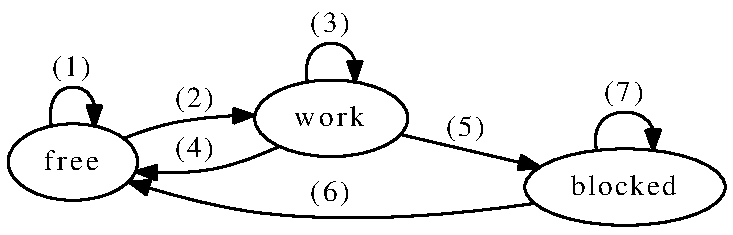
\includegraphics[width=\textwidth]{rules.pdf}
    \caption{Схема работы блока}
    \label{rules}
\end{figure}

Работу каждого блока можно схематично изобразить в виде автомата, см. рисунок \ref{rules}.

Поясним эти правила. Каждое правило \eqref{freetofree} --- \eqref{blocktoblock} описывает условие перехода в конечном автомате на рисунке \ref{rules}.

Правила \eqref{freetofree} и \eqref{freetostart} говорят о поведении свободного блока --- если блок может запуститься из его текущего состояния $s^t_v$
(то есть хватает данных на портах для какого-либо перехода), то он поглощает данные $\omega^t_{I, v}$ и
начинает некий переход $\pi^{t+1}_v$ из текущего состояния, иначе остается свободным дальше.

Тройка правил \eqref{worktowork}, \eqref{worktofree} и \eqref{worktoblock} описывают поведение работающего блока $v$. Если множество $\phi^t$ не содержит рассматриваемый блок,
он продолжает работу. Иначе, возможны два варианта: либо блок может завершиться и испустить данные $\zeta^t(v)$ (то есть ребра $\Delta_{O^t_v, v}$, связанные с испускаемыми портами $O^t_v$, свободны), то блок благополучно завершает работу $\xi^{t + 1}(v)$ и испускает данные ($\omega^t_{O, v}$), либо блок переходит в состояние блокировки до момента, когда требуемые ребра освободятся, которое описывается правилами \eqref{blocktofree} и \eqref{blocktoblock}.

Заметим, что мы специально различаем состояния блокировки и работы, хотя можно было бы считать, что заблокированный блок просто работает дополнительное время.
Состояние блокировки отличается тем, что блок в этом состоянии не требует вычислительных ресурсов, что будет важно в дальнейшем.

Заметим, что в правилах поведения потока данных сразу видны все неопределенности, о которых говорилось ранее --- перед запуском блока, определяется переход, который будет совершать блок, вместе с набором поглощаемых портов и ребра с которых эти данные будут поглащены. Подробнее мы будем рассматривать эти неопределенности далее.

\section{Анализ модели}
\subsection{Построение конечного автомата Мили по программе блока}
Введенная выше модель оперирует с упрощенными описаниями алгоритмов блоков --- каждый алгоритм заменяется на описывающий его качественное поведение автомат Мили.
Вначале опишем вид программы для блока.

Каждый блок реализует поведение так называемого актора (actor).
Перед запуском потока данных, среда запуска опрашивает каждый блок на начальные возможные наборы входных портов.
В конце запуска блок декларирует наборы входных портов для следующего запуска и выписывает результаты своей работы в определенные им порты.
Понятно, что после каждого шага работы, блок изменяет значение своих внутренних переменных (то есть свое состояние). Так как нас интересует лишь качественное поведение блока,
а значит лишь классы внутренних состояний, характеризующиеся множествами наборов входных и выходных портов,
начав работу из которых (т.е. поглотив данные из какого-либо набора входных портов из заданного множества)
при любых входных данных блок испустит данные по какому-либо набору выходных потров из заданного множества.
Отметим, что для дальнейшего рассмотрения будет удобно ввести особое состояние автомата Мили $\initial$, в котором все внутренние переменные равны начальным значениям.
На практике это состоянии означает, что блок фактически не использует выделенные ему ресурсы памяти и его можно быстро перенести при надобности на другой вычислительный узел.

Так как вычисление автомата Мили для программы любого блока машиной крайне ресурсоемкая операция, требующая полного анализа поведения при всех возможных входных данных,
что неосуществимо в реальности, приведем лишь неформальный алгоритм построение автомата Мили.

\end{document}